\section{Methods}

In order to demonstrate that the DISHTINY platform selects for detectable hierarchical transitions in individuality, we performed experiments where cell-like organisms evolved parameters to control manually-designed strategies such as resource-sharing, reproductive decision-making, and apoptosis.
We will first cover the design of the DISHTINY platform and then describe the simple cell-like organisms we used to evaluate the platform.

\subsection{DISHTINY}

\begin{figure*}[t]
\begin{center}
\includegraphics[width=2.0\columnwidth]{img/explanatory}
\caption{
\textbf{Activation signaling, and net resource collection for three different-sized same-channel networks during a resource wave event.}
At the top, a resource wave is depicted propagating over three updates and then ceasing for four updates (left to right).
In row $a$, a small two-cell channel-signaling group (far left, in green) is activated; tracking the resource wave (top) yields a small net resource harvest (far right).
In row $b$, an intermediate-sized 13-cell channel-signaling group yields a high net resource harvest.
Finally, in row $c$, a large 29-cell channel-signaling group incurs a net negative resource harvest.
In rows $a$, $b$, and $c$, dark purple indicates the active state, light purple indicates the quiescent state, and white indicates the ready state.
}
\label{fig:explanatory}
\end{center}
\end{figure*}


DISHTINY allows cell-like organisms to replicate across a toroidal grid.
Over discrete timesteps (``updates''), the cells can collect a continuous-valued resource.
Once sufficient resource has been accrued, cells may pay $3.0$ resource to place a daughter cell on an adjoining tile of the toroidal grid (i.e., reproduce), replacing any existing cell already there.
As cells reproduce, they can choose to include offspring in the parent's cooperating ``signaling channel'' group or force offspring to create a new cooperating ``signaling channel'' group.

As shown at the top of Figure \ref{fig:explanatory}, resources appear at a single point then spread outwards update-by-update in a diamond-shaped wave, disappearing when the expanding wave reaches a predefined limit.
Cells must be in a costly ``activated'' state to collect resource as it passes.
The cell at the starting position of a resource wave is automatically activated, and will send the activate signal to neighboring cells on the same signaling channel.
The newly activated cells, in turn, activate their own neighbors registered to the same signaling channel.
Neighbors registered to other signaling channels do not activate.
Each cell, after sending the activation signal, enters a temporary quiescent state so as not to reactivate from the signal.
In this manner, cells sharing a signaling channel activate in concert with the expanding resource wave.
As shown Figure \ref{fig:explanatory}$a,b$, the rate of resource collection for a cell is determined by the size and shape of of its same-channel signaling network;
small or fragmented same-channel signaling networks will frequently miss out on resource as it passes by.

Each cell pays a resource cost when it activates.
This cost is outweighed by the resource collected such that cells that activate in concert with a resource wave derive a net benefit.
Recall, though, that resource waves have a limited extent.
Cells that activate outside the extent of a resource wave or activate out of sync with the resource wave (due to an indirect path from the cell that originated the signal) pay the activation cost but collect no resource.
Cells that frequently activate erroneously use up their resource and die.
In our implementation, organisms that accrue a resource debt of $-5$ or greater are killed.
This erroneous activation scenario is depicted in Figure \ref{fig:explanatory}$c$.

In this manner, ``Goldilocks'' --- not to small and not too big --- signaling networks are selected for.
Based on a randomly chosen starting location, resource wave starting points (seeds) are tiled over the toroidal grid such that the extents of the resource waves touch, but do not overlap.
All waves start and proceed synchronously;
when they complete, the next resource waves are seeded.
This process ensures that selection for ``Goldilocks'' same-channel signaling networks is uniformly distributed over the toroidal grid.

Cells control the size and shape of their same-channel signaling group through strategic reproduction.
Three choices are afforded: whether to reproduce at all, where among the four adjoining tiles of the toroidal grid to place their offspring, and whether the offspring should be registered to the parent's signaling channel or be given a random channel ID (in the range 1 to $2^{64}$).
The probability of channel collision is miniscule: $60 \times 60 \times 50100$ (the grid dimensions times the number of simulation updates) independent channel values will only collide with probability $1 \times 10^{-11}$.
No guarantees are made about the uniqueness of a newly-generated channel ID, but chance collisions are rare.

To ensure turnover of channel groups, a channel generation limit is enforced.
Each time a cell spawns a daughter cell sharing the same channel, the parent's channel generation counter is incremented and the daughter cell's channel generation counter is then initialized to match their  parent's counter.
Once the channel generation counter reaches a limit, in this implementation defined as the resource wave radius, daughter cells may no longer be endowed with the parent's channel ID; a new, randomly-drawn channel ID is assigned to daughter cells instead.

In these experiments, we worked with two alternate resource wave sizes.
Small resource waves extended a radius of four toroidal tiles.
Large resource waves extended a radius of 12 toroidal tiles.
For both treatments, activated cells netted $+2.0$ resource from a resource wave, but suffered an activation penalty of $-5.0$ if no resource was available.
Due to the different radii of resource waves on different levels, level one selects for small same-channel signaling networks and level two selects for large same-channel signaling networks.
Small resource waves support a same-channel group of at most around eight cells.
Large resource waves support a same-channel group of at most around 72 cells.

Channel IDs enable straightforward detection of an evolutionary transition in individuality.
Because common channel IDs may only arise systematically through inheritance, common channel IDs indicate a close hereditary relationship in addition to a close cooperative relationship.
Because new channel IDs arise first in a single cell, same-channel signaling networks are reproductively bottlenecked, ensuring meaningful reproductive lineages at the level of the same-channel signaling network.
To recognize an evolutionary transition in individuality, we therefore evaluate
\begin{enumerate}
\item Do cells with the same channel ID choose to share resources (e.g., cooperate)?
\item Is there division of reproductive labor between members of the same channel (e.g., do cells at the interior of a network cede reproduction to those at the periphery?)
\end{enumerate}
By design, DISHTINY selects for resource sharing and reproductive cooperation because these behaviors help grow and maintain the same-channel signaling networks necessary for rapid resource collection, so same-channel groups that cooperate will tend to outcompete those that do not.

\subsection{Organisms}

\begin{figure*}[t]
\begin{center}
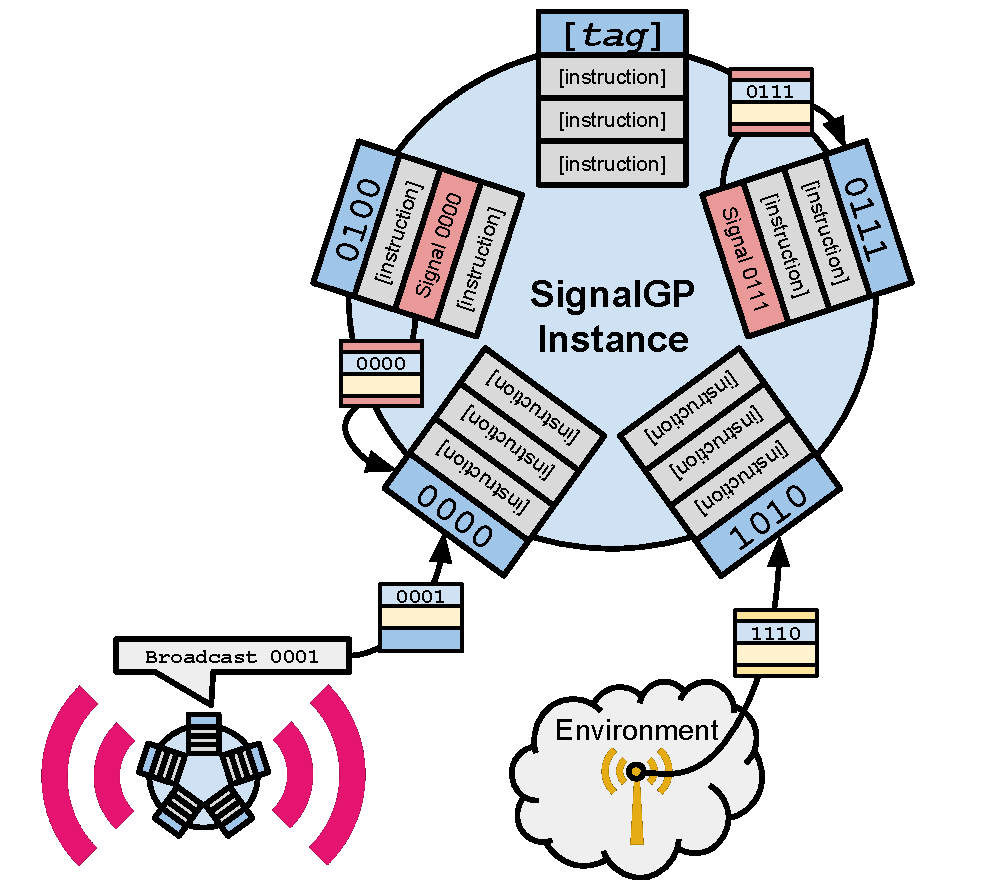
\includegraphics[width=\columnwidth]{img/signalgp-cartoon}%
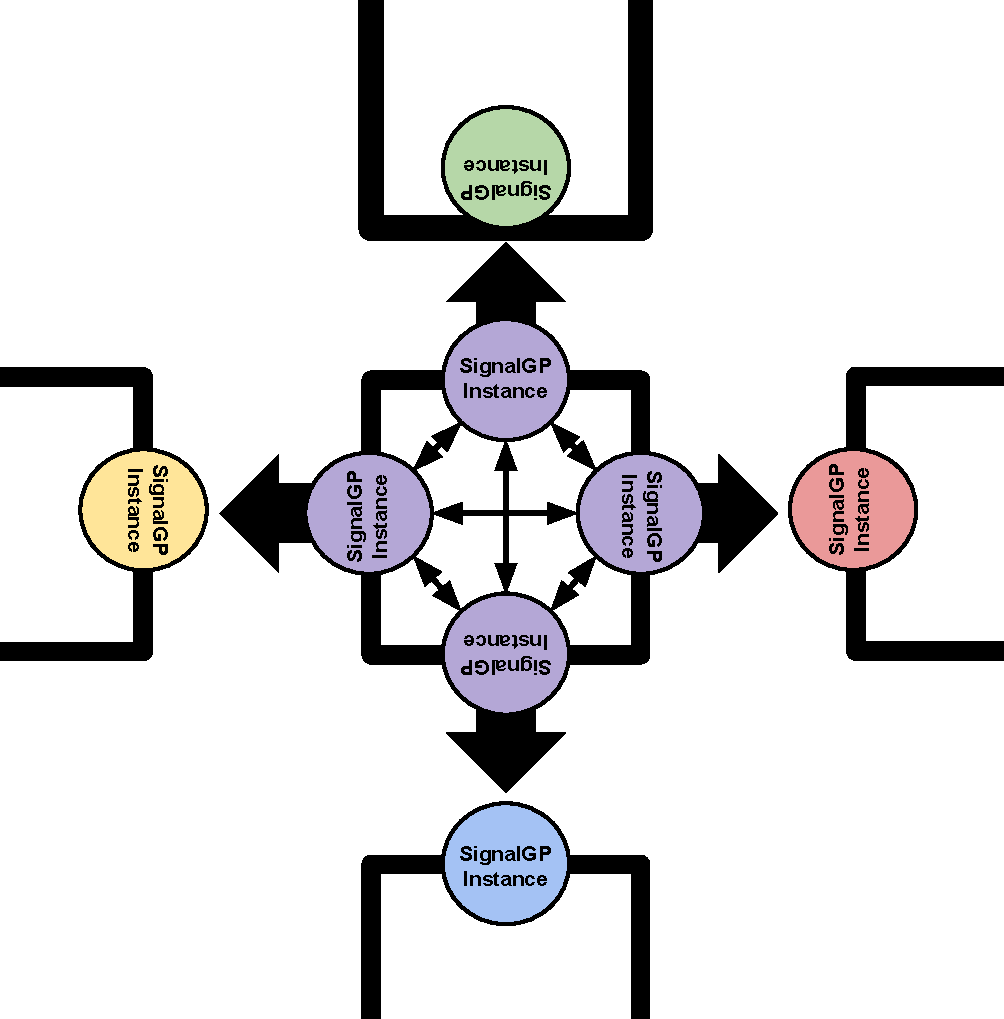
\includegraphics[width=\columnwidth]{img/dishtinygp-cartoon}
\caption{TODO}
\label{fig:signalgp-dishtinygp}
\end{center}
\end{figure*}


We performed our experiments using cell-level digital organisms controlled by evolving SignalGP programs.
SignalGP is genetic programming framework designed around the event-driven programming paradigm \cite{lalejini2018evolving}.
SignalGP programs are collections of independent procedural functions, each equipped with a bit-string tag.
A function is triggered by a signal with affinity that maximally and sufficiently matches its tag.
(A binding threshold of 0.5 was used in these experiments).
Signals may be generated by the environment, received as messages from other agents, or triggered internally by function execution.
Signals, and the ensuing chains of procedural execution they give rise to, are processed pseudo-concurrently by sixteen virtual CPUs.
Fifty virtual CPU cycles are carried out during each update.
Figure \ref{fig:signalgp} schematically depicts a single SignalGP instance.

Previous work evolving digital organisms to perform grid-based tasks in which a single computational instance designates which direction to act in via an explicit cardinal ``facing'' state or output \cite{goldsby2014evolutionary, goldsby2018serendipitous, grabowski2010early, biswas2014causes, lalejini2018evolving}.
However, in our work each cell employs four instances of SignalGP: one ``facing'' each cardinal direction.
These computational instances all execute the same SignalGP program but are otherwise decoupled and may follow independent chains of execution.
These instances execute single round robin in an order that is randomly drawn at the outset of each update.
The single SignalGP program that is mirrored across the cell's computational instances represents the cell's genome.
Mutation, described in more detail below, is applied to a faction of daughter cells at birth.

Instances within a cell may send intracellular messages to one another or intercellular messages to a neighboring cell.
Intercellular messages are received by the SignalGP instance that faces the sending cell.
Figure \ref{fig:dishtinygp} schematically depicts the configuration of the four SignalGP instances that constitute a single DISHTINY cell as well as the instances of neighboring cells that receive extracellular messages from the focal cell.

A combination of event-driven environmental triggers and procedural instruction-based sensors detailed in the following two subsections.

\subsection{Instruction Library}

In addition to the generic arithmetic, logic, and program flow instructions in the default SignalGP instruction set, which is detailed in \cite{lalejini2018evolving}, we define the following instructions.
Instructions that involve an extracellular neighbor default to the cell that the executing SignalGP instance is facing, but may be modified by a register-based argument.
Many instructions in the listing are provided in several variants, which are detailed in the accompanying description.

\begin{itemize}
\item \textbf{RNG Draw}
Draw a random value between 0.0 and 1.0 from on board random number generator and store result in register.
\item \textbf{Send/Broadcast Intracellular Message}
Send a message to a single other SignalGP instance within the cell or to all SignalGP instances (except the executing instance) within the current cell.
\item \textbf{Set Stockpile Reserve}
Mark twice the amount of resource as ineligible for sharing.
The amount may be modified by a register-based argument.
\item \textbf{Activate/Deactivate Intercellular Inbox}
Mark or unmark the intercellular inbox in a particular direction to refuse incoming messages.
At cell birth, the inbox is deactivated.
\item \textbf{Share Resource}
Send a proportion of the cell's stockpiled resource to a neighboring cell.
One instruction defaults to sending a large proportion of available resource (50\%) to the neighboring cell.
A second instruction defaults to sending a small proportion of available resource (5\%) to the neighboring cell.
The proportion of available resource can be adjusted by a register-based argument.
\item \textbf{Accept/Decline Sharing}
Mark the cell to decline resource sent by neighbors.
Declined resource is retained by the sending cell (with no resource lost).
Regardless of this instruction, cells with negative resource stockpiles automatically decline shared resource.
At birth, the cell is marked to accept sharing.
\item \textbf{Send/Broadcast Intercellular Message}
Send a message to a single cellular neighbor or to all cellular neighbors.
\item \textbf{Reproduce}
Attempt to spawn a child cell in a particular direction, paid for out of the parent cell's resource stockpile.
If sufficient resource is not available in the cell's stockpile, no resource is action is taken.
Variants of this instruction are defined for each channel ID inheritance level: from endowing the daughter cell with the parental channel IDs across all levels, to endowing the daughter cell with a new level-one channel ID but the parent's level-two channel ID, to endowing the daughter cell with all-new channel IDs.
If a channel generation counter limit has been reached, reproduction is simply attempted at the next highest level; even with channel generation counters maxed out, cells may generate offspring with all-new channel IDs.
\item \textbf{Pause Reproduction}
Pause cellular reproduction in a single direction for the remainder of the current update and for the entire next update.
Variants of this instruction pause reproduction at a certain wave/channel-signaling level or across all channel ID inheritance levels.
\item \textbf{Increase Channel Generation Counter}
Increases the cell's channel generation counter by one.
The amount the cell's generation counter is increased by can be adjusted by register-based argument.
\item \textbf{Apoptosis}
The cell is killed at the end of the current update.
Two variants are defined.
Under the conplete variant, the cell's channel ID partial and complete
\item \textbf{Designate/Revoke Heir} apoptosis 80\% of reproduction cost and own stockpile amount
\item \textbf{Query Own Stockpile}
Sets a designated register to the amount of resource present in the cell's stockpile.
\item \textbf{Query Own Channel Generation Counter} -Lev
This instruction sets a designated register to the value of the cell's channel generation counter.
A variant of this instruction is provided for each wave/channel-signaling level.
\item \textbf{Query ``Is Neighbor Live?''}
This instruction sets a designated register to 1 if the neighboring tile contains a live cell and 0 otherwise.
\item \textbf{Query ``Is Neighbor Channel Set?''}
This instruction sets a designated register to 1 if the neighboring tile contains active channel IDs and 0 otherwise.
\item \textbf{Query ``Is Neighbor My Cellular Child?''}
This instruction sets a designated register to 1 if the neighboring cell is the daughter of the querying cell and 0 otherwise.
\item \textbf{Query ``Is Neighbor My Cellular Parent?''}
This instruction sets a designated register to 1 if the neighboring cell is the parent of the querying cell and 0 otherwise.
\item \textbf{Query ``Does Neighbor's Channel ID Match Mine?''}
This instruction sets a designated register to 1 if the neighboring cell has the same channel ID as the querying cell and 0 otherwise.
A variant of this instruction is provided for each wave/channel-signaling level.
\item \textbf{Query ``Does Neighbor's Channel ID Descend From Mine?''}
This instruction sets a designated register to 1 if the neighboring cell's highest-level channel ID is different from the querying cell's highest-level channel ID, but is descended from the querying cell's channel ID.
This instruction allows a querying cell to sense whether its neighbor is a member of a same-channel group that is a propagule of the querying cell's same-channel group.
\item \textbf{Query ``Does My Channel ID Descend From Neighbor's?''}
This instruction sets a designated register to 1 if the querying cell's highest-level channel ID is different from the neighboring cell's highest-level channel ID, but is descended from the neighboring cell's channel ID.
\item \textbf{Query Neighbor's Channel ID}
This instruction sets a designated register to the neighbor's channel ID.
\item \textbf{Query Neighbor's Stockpile}
This instruction sets a designated register to the amount of resource present in the neighbor's stockpile.
\end{itemize}

\subsection{Event Library}

The activating affinity of each event is set at the outset of each experiment using a pseudo random number generator.

\begin{itemize}
\item \textbf{On Update}
This event is triggered at the outset of each simulation update.
\item \textbf{Facing Cellular Child}
This event is triggered at the outset of an update if the SignalGP instance is facing a neighboring cell that is the querying cell's daughter.
\item \textbf{Stockpile Debt}
This event is triggered at the outset of an update if the amount of resource in a cell's stockpile is negative.
\item \textbf{Neighbor's Channel ID Matches Mine} defined per level
This event is triggered at the outset of an update if a SignalGP instance is facing a neighbor cell that shares its channel ID.
A different event is provided for each resource wave/channel-signaling level.
\item \textbf{Neighbor's Channel ID Descends From Mine}
This event is triggered at the outset of an update if the neighboring cell's highest-level channel ID is different from the querying cell's highest-level channel ID, but is descended from the querying cell's channel ID.
This event allows a querying cell to sense whether its neighbor is a member of a same-channel group that is a propagule of the querying cell's same-channel group.
\end{itemize}

\subsection{Treatments}

In this work, we explore two experimental parameters:
\begin{enumerate}
\item mutational load and
\item resource wave size.
\end{enumerate}

The default SignalGP mutational parameter settings are as follows,
\begin{itemize}
\item per-bit mutation rate of tag bit flips: 0.005 (\verb|TAG_BIT_FLIP__PER_BIT|),
\item per-instruction/argument substitution rate: 0.005 (\verb|INST_SUB__PER_INST|),
\item per-instruction/argument substitution rate: 0.005  (\verb|ARG_SUB__PER_ARG|),
\item per-instruction insertion mutation rate: 0.005 (\verb|INST_INS__PER_INST|),
\item per-instruction deletion mutation rate: 0.005 (\verb|INST_DEL__PER_INST|),
\item per-function rate of slip mutations: 0.05 (\verb|SLIP__PER_FUNC|)
\item per-function rate of function duplications: 0.05 (\verb|FUNC_DUP__PER_FUNC|), and
\item per-function rate of function deletions: 0.05 (\verb|FUNC_DEL__PER_FUNC|).
\end{itemize}

We use five mutational load treatments, numbered one through five in increasing order of severity,
\begin{enumerate}
\item default SignalGP mutational parameter settings with mutations only applied to 5\% of offspring,
\item default SignalGP mutational parameter settings with mutations only applied to 25\% of offspring,
\item default SignalGP mutational parameter settings with mutations applied to 100\% of offspring,
\item $3\times$ SignalGP mutational parameter settings with mutations applied to 100\% of offspring, and
\item $12\times$ SignalGP mutational parameter settings with mutations applied to 100\% of offspring.
\end{enumerate}

We use two resource wave size treatments,
\begin{itemize}
\item ``small'' resource wave (radius four) and
\item ``large'' resource wave (radius 12).
\end{itemize}

We mix and match these two experimental parameters (mutational load and resource wave size) into ten total treatments.
For each treatment, 20 replicate evolutionary runs lasting 50k updates were performed.
Each evolutionary run required on the order of four hours of compute time.

\subsection{Implementation}

We implemented our experimental system using the Empirical library for scientific software development in C++, available at \url{https://github.com/devosoft/Empirical}.
The code used to perform and analyze our experiments, our figures, data from our experiments, and a live in-browser demo of our system is available via the Open Science Framework at \url{https://osf.io/js5a3/}.
